\documentclass[tikz]{standalone}
\usepackage[utf8x]{inputenc}
\usepackage{tikz}
\usetikzlibrary{patterns}
\begin{document}
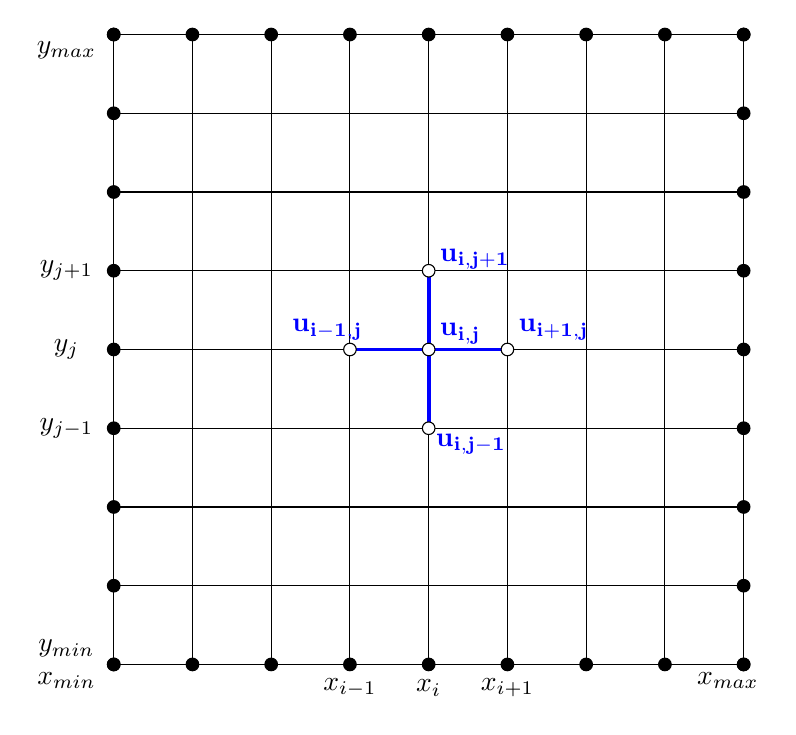
\begin{tikzpicture}

	\foreach \x in {0,1,2,3,4,5,6,7,8}
		\draw (0, \x) -- (8, \x);
	
	\foreach \x in {0,1,2,3,4,5,6,7,8}
		\draw (\x, 0) -- (\x, 8);
	
	\foreach \x in {0,1,2,3,4,5,6,7,8}
		\foreach \y in {0,8}
			\draw [fill](\x,\y) circle (0.08);
			
	\foreach \x in {0,1,2,3,4,5,6,7,8}
		\foreach \y in {0,8}		
			\draw [fill](\y,\x) circle (0.08);
	
	\draw(-0.6, -0.2) node {$x_{min}$};
	\draw(-0.6, 0.2) node {$y_{min}$};
	\draw (7.8, -0.2) node {$x_{max}$};
	\draw (-0.6, 7.8) node {$y_{max}$};

	\draw(-0.6, 3) node {$y_{j - 1}$};	
	\draw(-0.6, 4) node {$y_{j}$};
	\draw(-0.6, 5) node {$y_{j + 1}$};

	\draw(3, -0.3) node {$x_{i - 1}$};	
	\draw(4, -0.3) node {$x_{i}$};
	\draw(5, -0.3) node {$x_{i + 1}$};

	\draw [line width = 0.5mm, blue] (4,4) -- (4,5) node [right, yshift=0.15cm] {$\mathbf{u_{i, j + 1}}$};
	\draw [line width = 0.5mm, blue] (4,3) -- (4,4) node [right, xshift=-0.05cm, yshift=-1.2cm] {$\mathbf{u_{i, j - 1}}$};
	\draw [line width = 0.5mm, blue] (3,4) -- (4,4) node [left, xshift=-0.7cm, yshift =0.25cm] {$\mathbf{u_{i - 1, j}}$};
	\draw [line width = 0.5mm, blue] (4,4) -- (5,4) node [right, yshift =0.25cm] {$\mathbf{u_{i + 1, j}}$};
	\draw [blue] (4.4,4.2) node {$\mathbf{u_{i, j}}$};

	
	
	\draw(3,4) [fill=white] circle (0.08);	
	\draw(4,4) [fill=white] circle (0.08);
	\draw(5,4) [fill=white] circle (0.08);
	
	\draw(4,3) [fill=white] circle (0.08);	
	\draw(4,5) [fill=white] circle (0.08);

\end{tikzpicture}
\end{document}